\documentclass{article}
\usepackage[utf8]{inputenc}
\usepackage[english]{babel}
\usepackage[a4paper,top=1.5cm,bottom=1.5cm,left=1.5cm,right=1.5cm,%
bindingoffset=0mm]{geometry}
\usepackage{amssymb}
\usepackage{amsmath}
\newtheorem{prop}{Proposition}
\newtheorem{lemma}{Lemma}
\newenvironment{proof}[1][Proof]{\begin{trivlist}
\item[\hskip \labelsep {\bfseries #1}]}{\end{trivlist}}
\newcommand{\qed}{\nobreak \ifvmode \relax \else
      \ifdim\lastskip<1.5em \hskip-\lastskip
      \hskip1.5em plus0em minus0.5em \fi \nobreak
      \vrule height0.75em width0.75em depth0em\fi}
\usepackage{tikz}
\usepackage{graphicx}
%\graphicspath{{./Figures/}}
\def \ourFigPath {../../} % this should move up two steps but it isn't working 
% . = current directory
 % .. = parent directory
\usepackage{rotating}
\usepackage{float}
\linespread{1.3}
\raggedbottom




%
\font\reali=msbm10 at 12pt
% subsets of real numbers
\newcommand{\real}{\hbox{\reali R}}
\newcommand{\realp}{\hbox{\reali R}_{\scriptscriptstyle +}}
\newcommand{\realpp}{\hbox{\reali R}_{\scriptscriptstyle ++}}
\newcommand{\R}{\mathbb{R}}
\DeclareMathOperator{\E}{\mathbb{E}}
%

\title{Discussion of Results}
\author{Marco Brianti\\Laura Gati}
\date{22 Nov 2017}

\begin{document}

\maketitle

\subsection*{Shares of FEV of TFP}

\

\textbf{Differenced relative prices (inflation of IT price index over CPI-inflation)}

IT: 51.60\%

\noindent News: 19.63\%

\

 \textbf{Log level of capital prices (differencing here seems to overdo it)}

IT: 28.47\%

\noindent News: 28.31\%



\newpage
\subsection*{IRFs - ratio of inflations (i.e relative prices)}

\begin{figure}[h!]
\centering
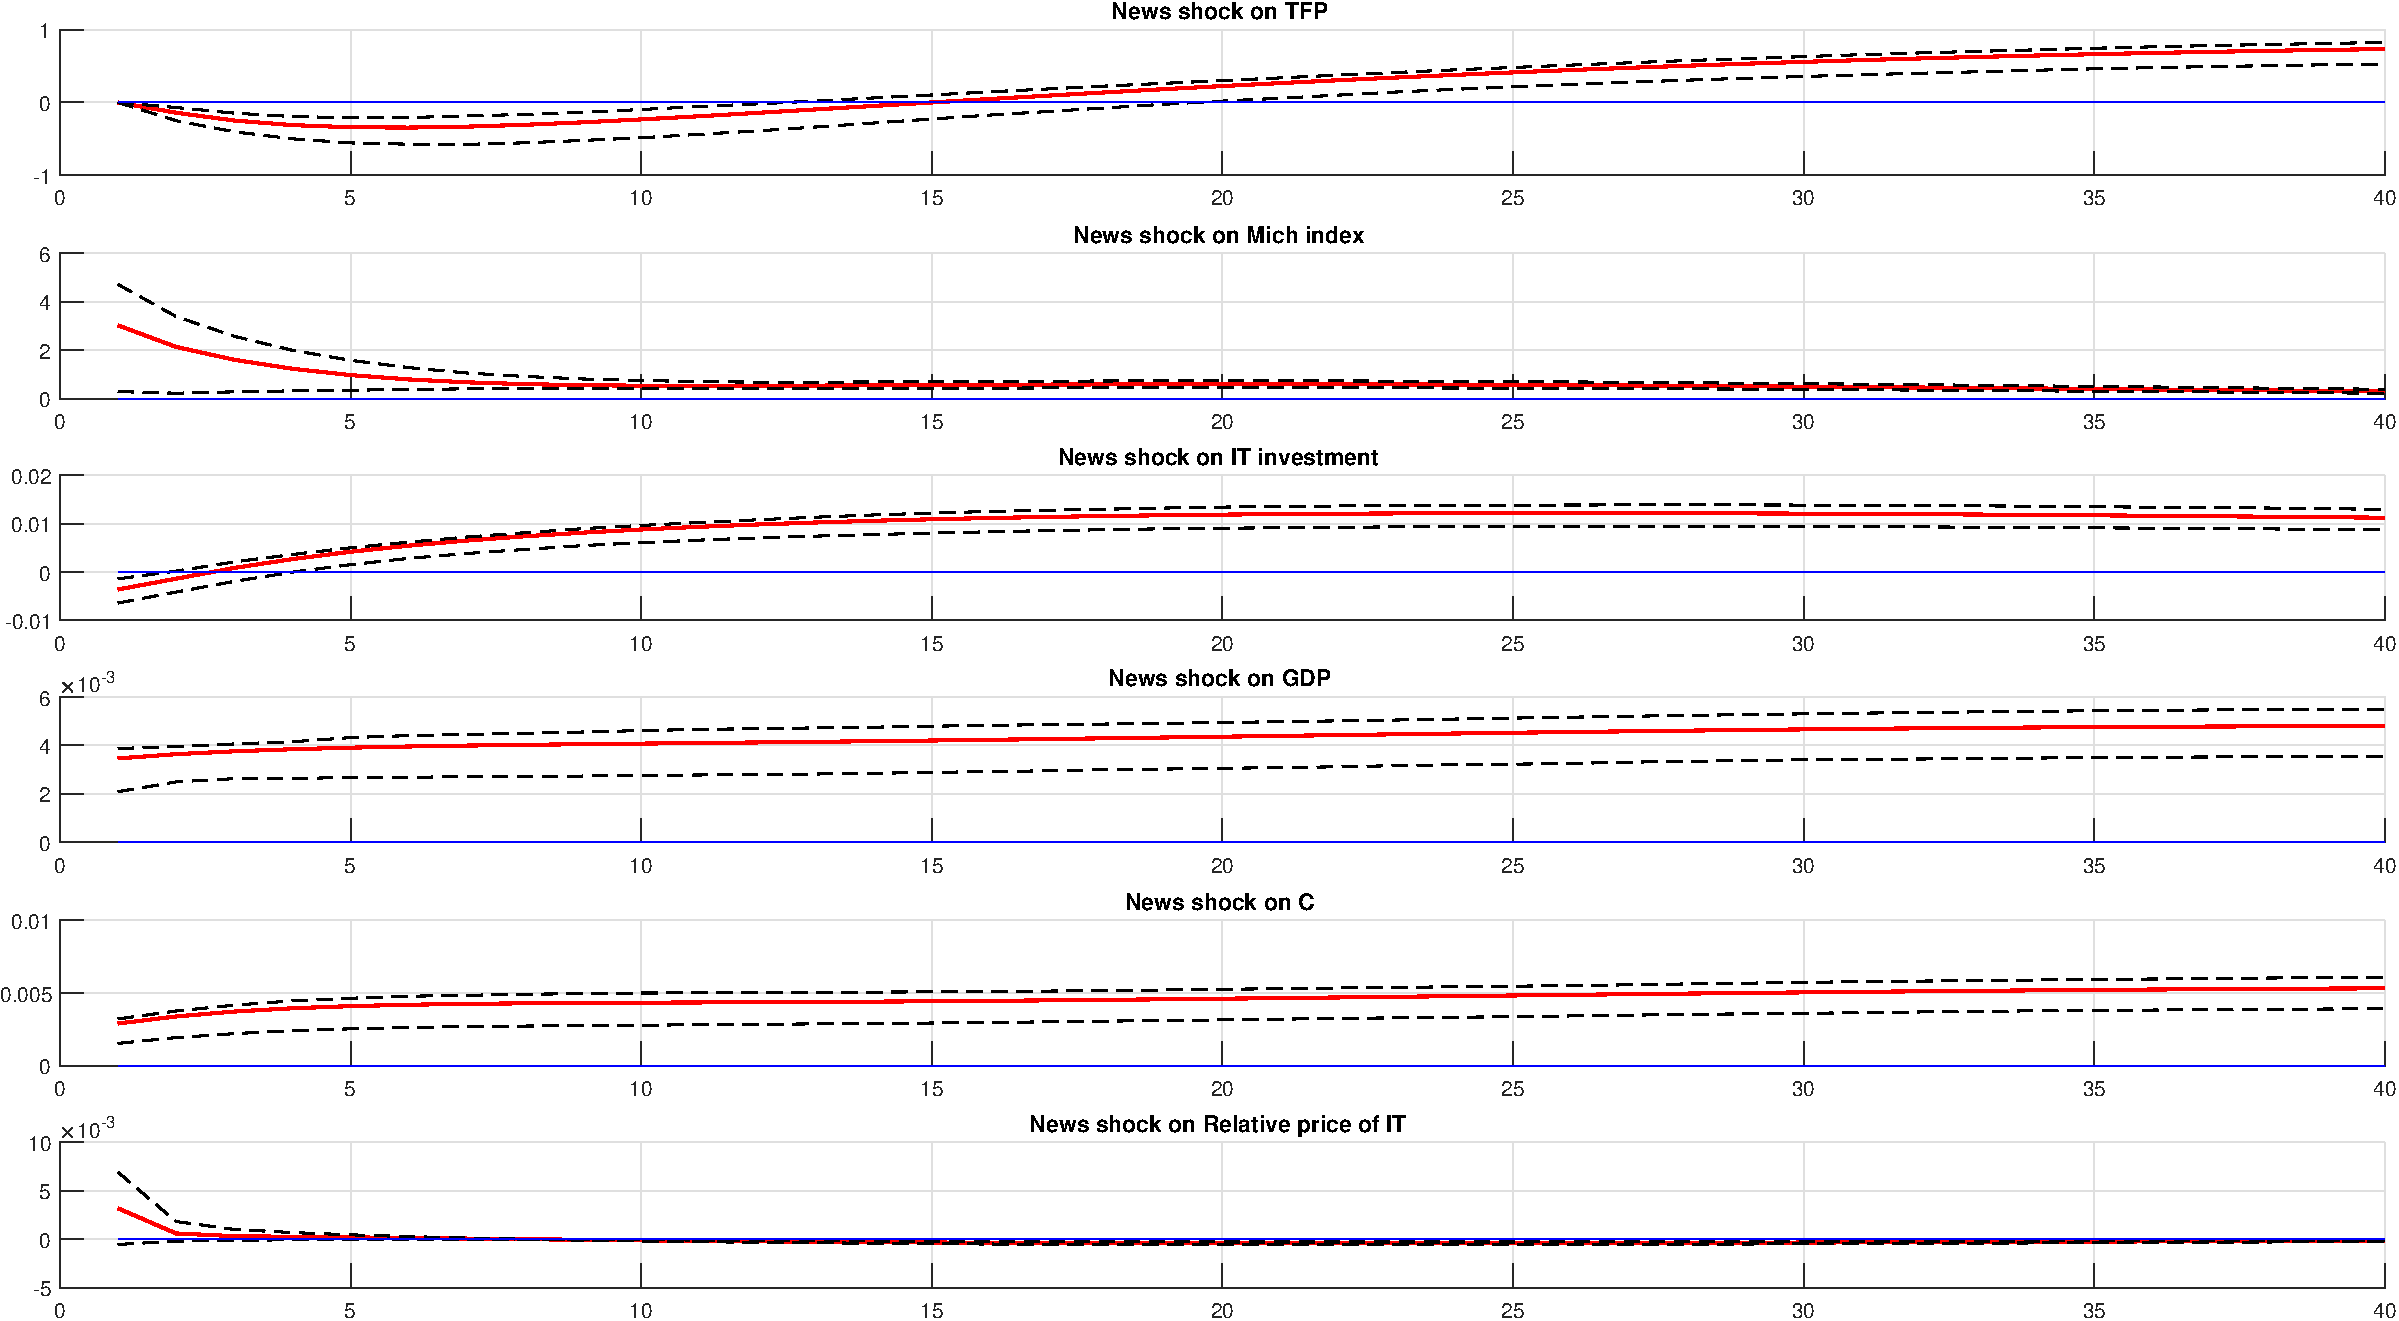
\includegraphics[scale=0.4]{\ourFigPath Figures/fig_News_shock_Ryan_two_stepsID_20-Nov-2017_12_24_34}
\caption{News shock - ratio of inflations}
\end{figure}

\begin{figure}[h!]
\centering
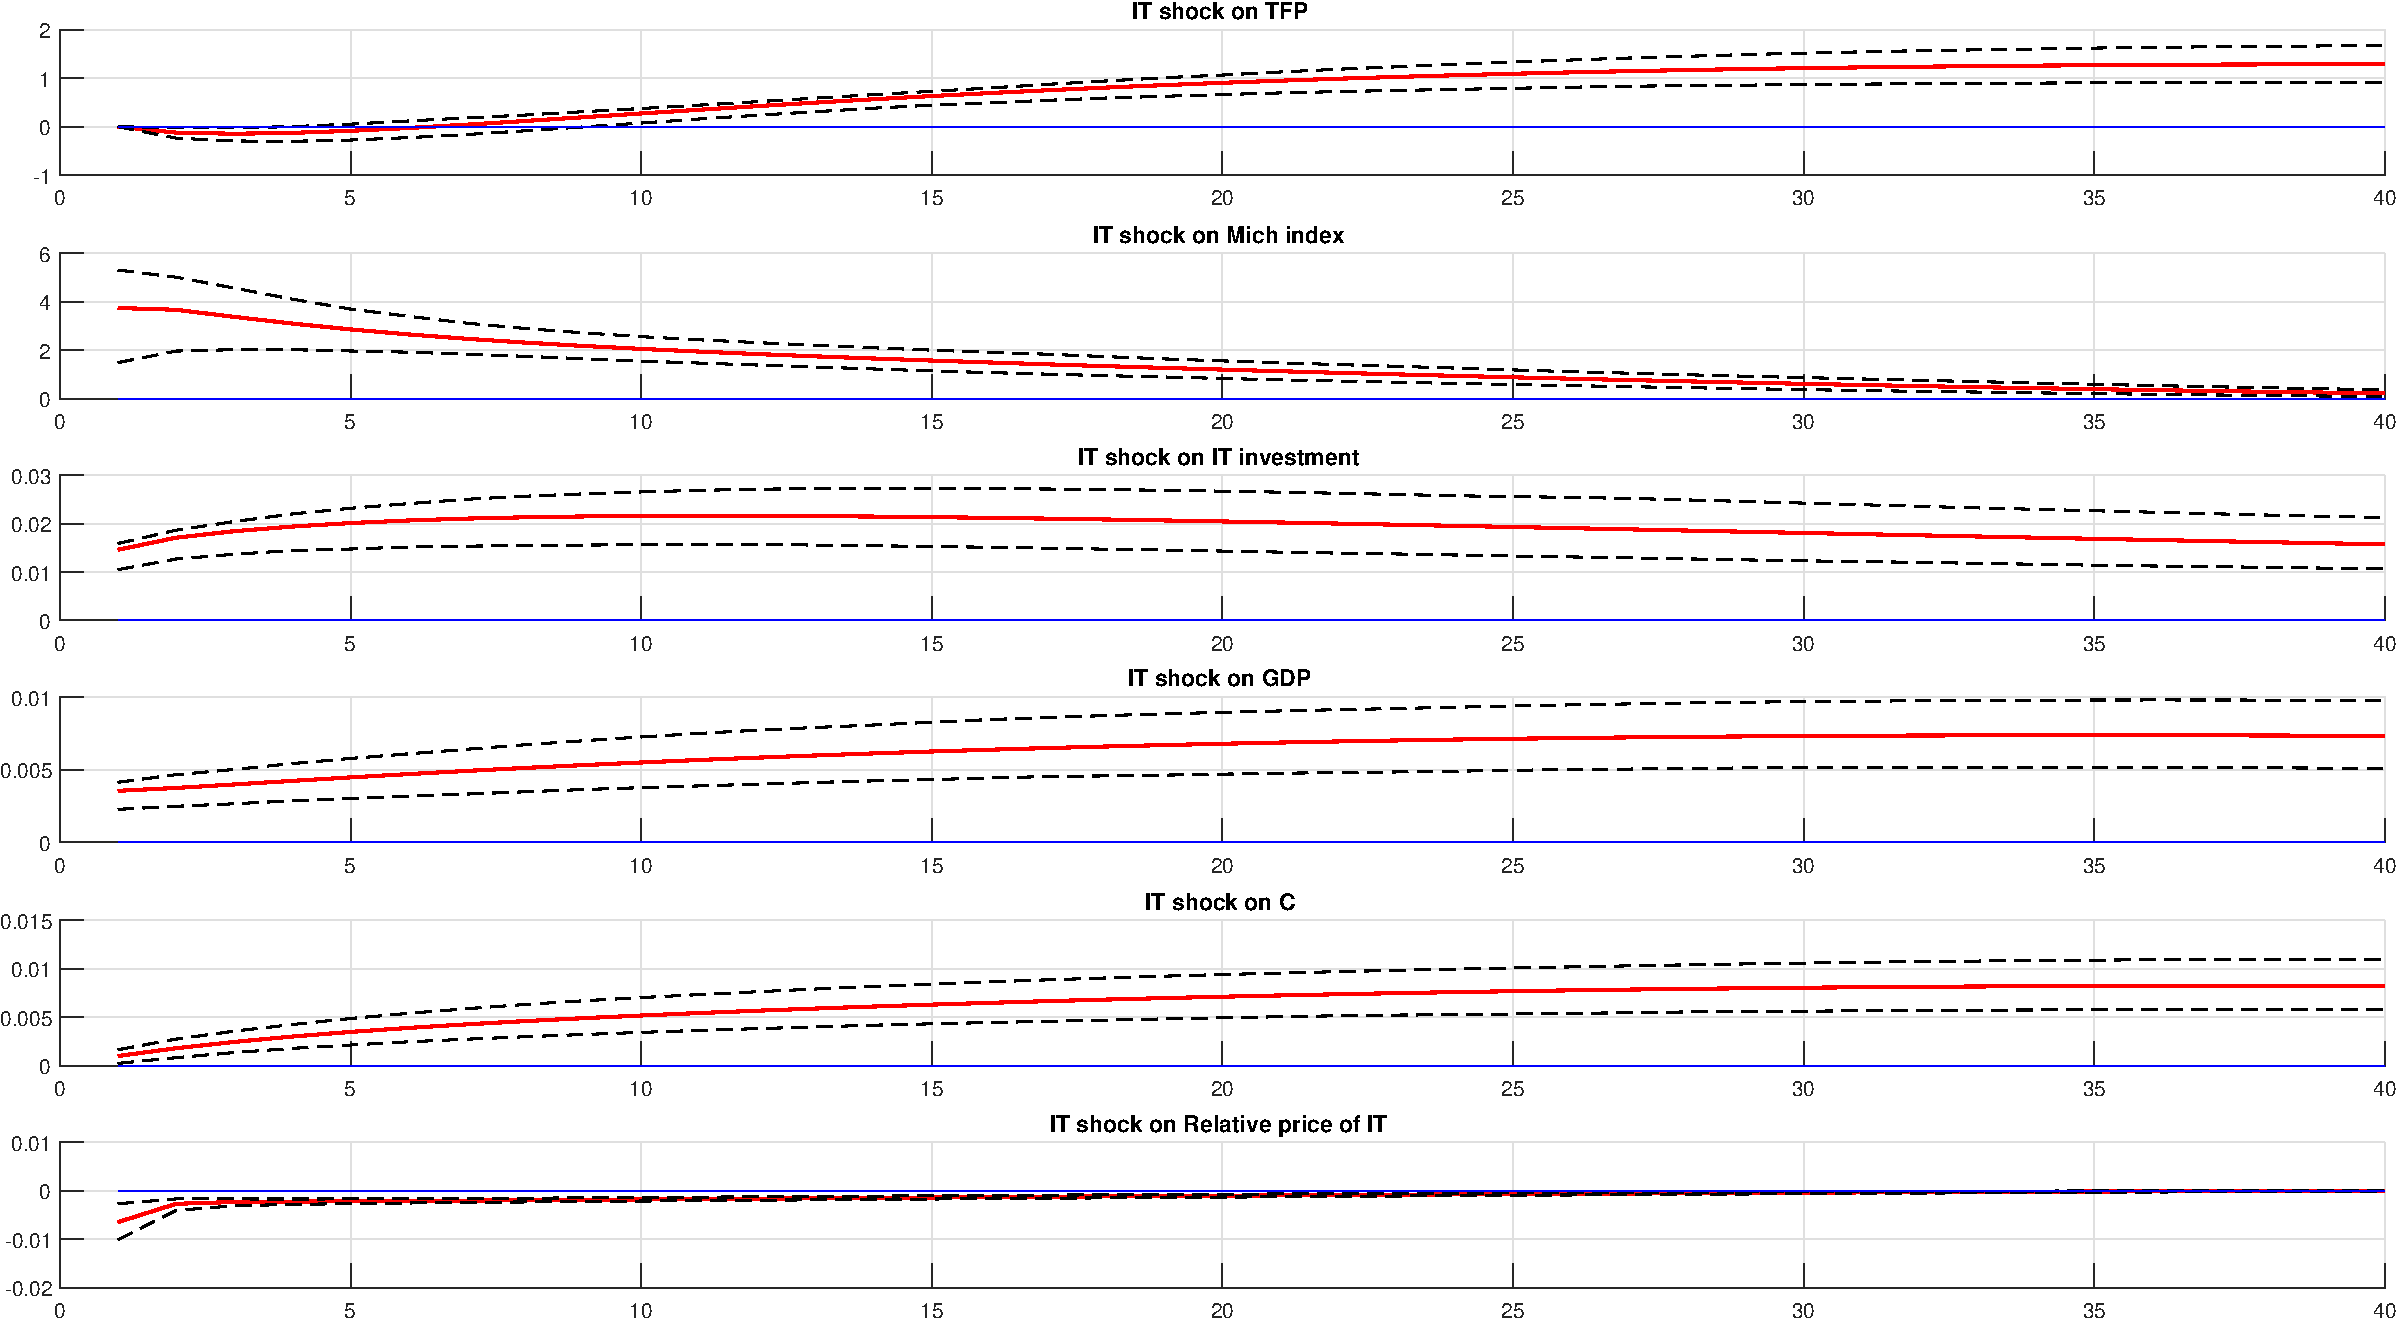
\includegraphics[scale=0.4]{\ourFigPath Figures/fig_IT_shock_Ryan_two_stepsID_20-Nov-2017_12_24_39}
\caption{IT shock - ratio of inflations}
\end{figure}

%%%%%
\newpage
\subsection*{IRFs - log level of capital prices}

\begin{figure}[h!]
\centering
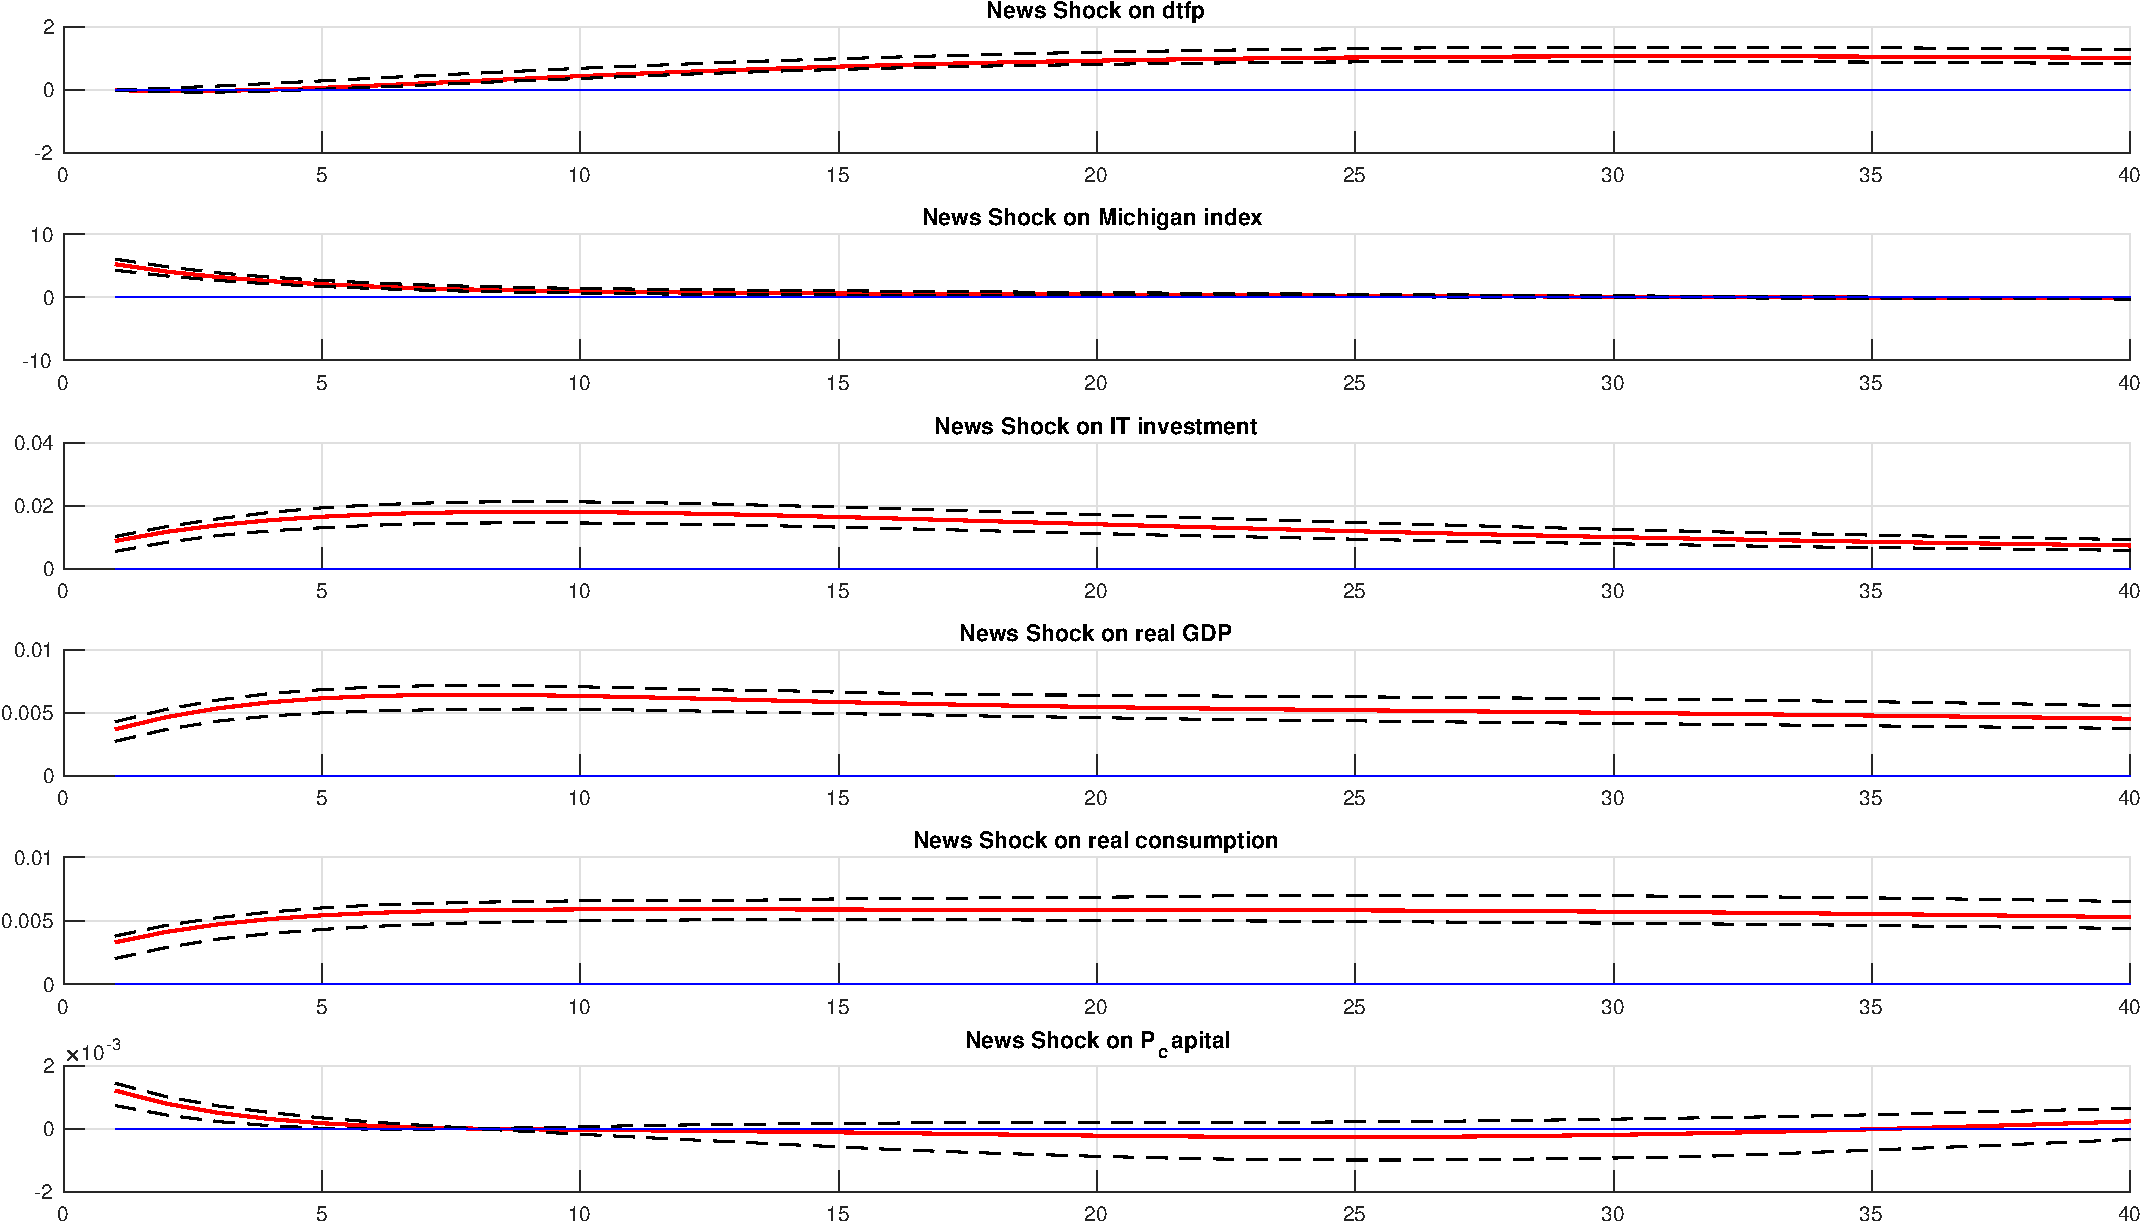
\includegraphics[scale=0.4]{\ourFigPath Figures/fig_News_Shock_Ryan_two_stepsID_21-Nov-2017_11_35_24}
\caption{News shock - log level of capital prices}
\end{figure}

\begin{figure}[h!]
\centering
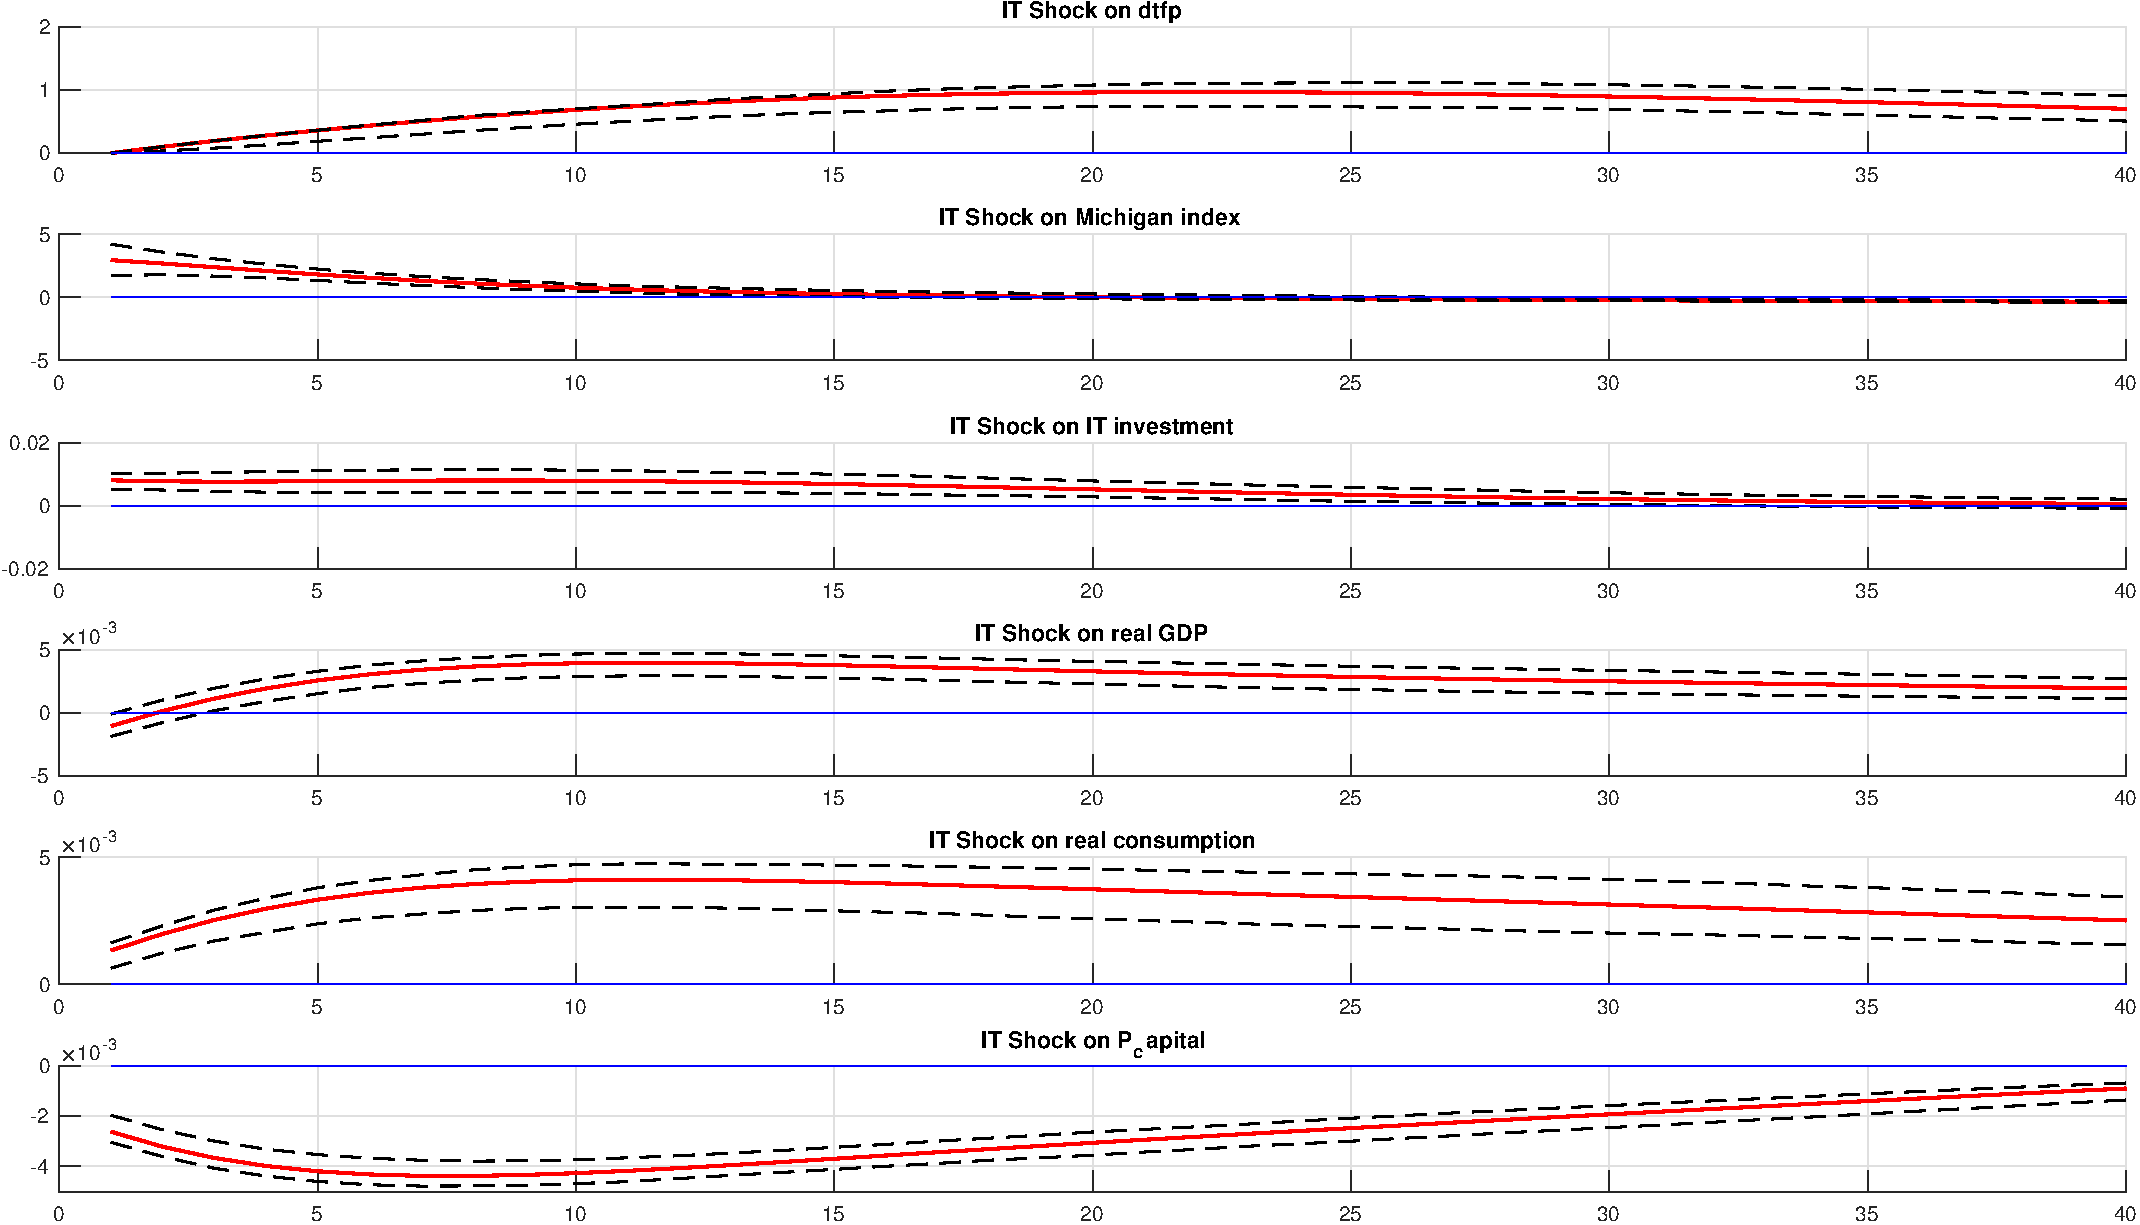
\includegraphics[scale=0.4]{\ourFigPath Figures/fig_IT_Shock_Ryan_two_stepsID_21-Nov-2017_11_35_27}
\caption{IT shock - log level of capital prices}
\end{figure}

\newpage
\subsection*{Recap and interpretation}

\begin{itemize}
\item One big motivation for the entire research project is the puzzling decrease in TFP growth, which - as we have also documented - started \emph{before} the Great Recession.
\item The sudden decrease in IT investment after the burst of the IT bubble around 2000-2002 coincides with this slowdown in TFP growth, which led us to investigate the effect of IT investment on TFP. 
\item We run a structural VAR to estimate the effect of an IT productivity shock on TFP and other main macroeconomic variables.
\item This identification poses a challenge because we need to confront the view that there is an endogenous channel in the evolution of TFP with the widely accepted view that TFP is driven by news. Since both are similar in the way they affect TFP only with lags, we need an additional restriction to disentangle the two.
\item The additional restriction we use is that news shocks should have no effect on relative IT prices at a certain (long) horizon, because they behave like demand shocks.
\item [] \textbf{What the results seem to suggest:}
\item [1)] News and IT shocks together explain more of the FEV of TFP than news does alone in Barsky \& Sims (around 70\% vs approximately 40\% in Barsky \& Sims). (Compare with capital prices specification too.)
\item [2)] News still explains a considerable fraction, but IT shocks explain more. (Compare with capital prices specification too.)
\item [] $\rightarrow$ we read this as evidence that both news and the endogenous channel via IT investment plays an important role in explaining TFP  over the business cycle and the medium run. 
\end{itemize}

\subsection*{Comments? Thoughts? Does this make sense to you? Is it presentable in its current form?}


\end{document}

